\documentclass[letterpaper, 12pt]{article}
\usepackage{fullpage,latexsym,amsthm,latexsym,amssymb}
\usepackage{amstext,amsfonts,amsmath,graphicx}
\usepackage{multicol}
\usepackage[usenames,dvipsnames]{color}
\usepackage{hyperref}
\usepackage{tikz}
\usepackage{graphicx}
\graphicspath{./}
\usetikzlibrary{automata, positioning}

\oddsidemargin = -0.5 in
\addtolength{\textwidth}{0.8in}
\addtolength{\textheight}{0.2in}

%% Theorem statements %%
% THEOREMS -------------------------------------------------------
\newtheorem{theorem}{Theorem}[section]
\theoremstyle{definition}
\newtheorem{definition}{Definition}
\numberwithin{equation}{section}
%% MISC DEFINITIONS %%%%%%%%%%%%%%%%%%%%%%%%%%%%%%%%%%%

\newcommand{\ignore}[1]{}

\DeclareMathOperator{\shuffle}{shuffle}

\newcommand{\N}{\mathbb N}
\newcommand{\abs}[1]{\left \vert #1 \right\vert}
\newcommand{\abi}[1]{\textcolor{Red}{#1}}
\newcommand{\qtrinfo}{CS181 Winter 2019}
\newcommand{\remove}[1]{}
\newcommand{\headnote}{
%\begin{multicols}{2}\small
\begin{itemize}
\item Please write your student ID \textbf{and the names of anyone you collaborated with} in the spaces provided and attach this sheet to the front of your solutions. \textbf{Please do not include your name anywhere since the homework will be blind graded.}
\item An extra credit of \textbf{5\%} will be granted to solutions written using \LaTeX. Here is one place where you can create \LaTeX documents for free: \url{https://www.overleaf.com/}. The link also has tutorials to get you started. There are several other editors you can use.
\item If you are writing solutions by hand, please write your answers in a neat and readable hand-writing.
\item Always explain your answers. When a proof is requested, you should provide a rigorous proof.
\item If you don't know the answer, write ``I don't know'' along with a clear explanation of what you tried. For example: ``I couldn't figure this out. I think the following is a start, that is correct, but I couldn't figure out what to do next. [[Write down a start to the answer that you are sure makes sense.]] Also, I had the following vague idea, but I couldn't figure out how to make it work. [[Write down vague ideas.]]'' At least 20\% will be given for such an answer.

Note that if you write things that do not make any sense, no points will be given.
\item The homework is expected to take anywhere between 8 to 14 hours. You are
advised to start early.
\item Submit your homework online on Gradescope. 
\end{itemize}
%\end{multicols}
}

\newcommand{\hwhead}[2]{
	\raggedleft{Student ID: \underline{\hspace{1.2in}304990072\hspace{1.25in}} \\ \medskip
              Collaborators: \underline{\hspace{3in}} \\ \medskip}
  \bigskip
  \begin{center}
  	{\LARGE{\qtrinfo \ -- Problem Set #1}}\\[0.3cm]
  	{\Large{Due #2}}
  \end{center}
  \bigskip
  \raggedright
  \headnote
}

%%%%%%%%%%%%%%%%%%%%%%%%%%%%%%%%%%%%%%%%%%%%%%%%%%%%%
\addtolength{\topmargin}{-1cm}
\addtolength{\textheight}{2cm}






\begin{document}
\hwhead{3}{Monday, February 11, 11:59 pm}


\begin{center}
\fbox{%
   \parbox{0.8\linewidth}{
Note: \textit{Suggested practice problems from the book: 2.4 and 2.5. Please, do not turn in solutions to problems from the book.}
   }
}
\end{center}

\newpage

\paragraph{Problem 1}
\subparagraph{} We can solve this problem by constructing a PDA $M = \{Q, \Sigma, \Gamma, \delta, q_1, F\}$. Since, $A, B$ are two regular languages, there exists two DFA $M_1 = \{Q_1, \Sigma_1, \delta_1, q_{01}, F_1\}, M_2 = \{Q_2, \Sigma_2, \delta_2 q_{02}, F_2\}$ that accepts $A$ and $B$ respectively. The idea is, we add $\epsilon$-transitions from all accept states of $M_1$ to the start state of $M_2$. For the first half of the PDA, $\delta = \delta_1$ for the state transitions, and push all symbols onto the stack. For the second part of the PDA, $\delta = \delta_2$ for the state transitions, and pop the top element of the stack if the element is not \$. The accepted states of $M_2$ have $\epsilon$-transitions to the accept state $q_{acc}$ we define for the PDA, the transition will only take place when the top element of the stack is \$. A more formal definition of the PDA is as follows: \\
\begin{itemize}
	\item $Q = Q_1 \cup Q_2 \cup \{q_1, q_{acc}\}$, $q_1$ is the new start state, $q_{acc}$ is the new accept state.
	\item $\Sigma = \Sigma_1 \cup \Sigma_2 \cup \{\epsilon\}$
	\item $\Gamma = \Sigma_1 \cup \{\epsilon, \$\}$
	\item $q_1$ is the new start state
	\item $F = q_{acc}$, $q_{acc}$ is the new accept state.
	\item $\delta(q, a, b) = 
	\begin{cases}
               (q_{01}, \$) &\textbf{if}\ q = q_1,\ a = \epsilon, b = \epsilon \\
               (\delta_1(q, a), a)  &\textbf{if}\ q \in Q_1,\ a \in \Sigma_1, b = \epsilon \\
               (q_{02}, \epsilon) &\textbf{if}\ q \in F_1, a = \epsilon, b = \epsilon \\
               (\delta_2(q, a), \epsilon)  &\textbf{if}\ q \in Q_2,\ a \in \Sigma_2, b \in \Sigma_1 \\
               (q_{acc}, \epsilon) &\textbf{if}\ q \in F_2, a = \epsilon, b = \$
    \end{cases}$\\~\\~\\
\end{itemize}
The PDA is as follows: \\
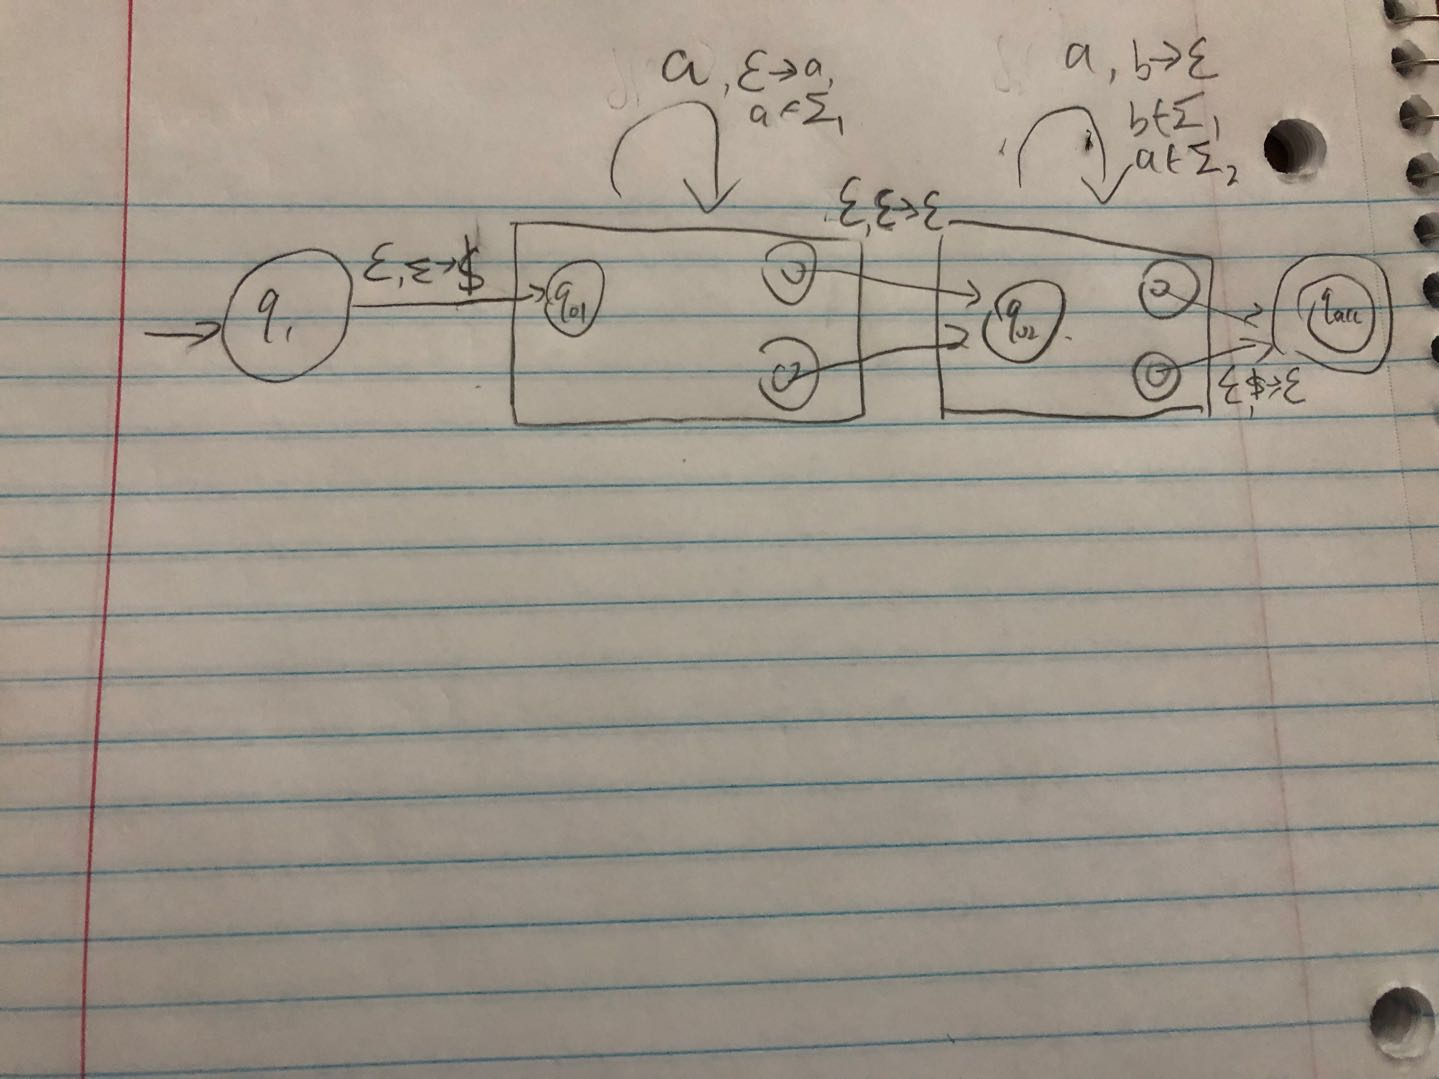
\includegraphics[scale=0.2]{PDA_1}

Suppose $s \in A\nabla B$, $M$ will begin in $q_1$ and we can have $\epsilon$-transition into $q_{01}$ by pushing  \$ onto the stack. After processing the first part of the string, we end up in one of the accept states in $M_1$, with the stack contains the full string $x$. Then we can have a $\epsilon$-transition into $q_{02}$ without modifying the stack. After processing the remaining part of string $s$, we end up in one of the accept states of $M_2$, and since $s \in A\nabla B$, $|x| = |y|$, the stack only contains a \$ symbol. Then the final $\epsilon$-transition will pop the \$ symbol and lead $M$ into its accept state $q_{acc}$. Hence, $A\nabla B \subseteq L(M)$. \\~\\

Suppose $s$ is accpeted by $M$. The only possible transitions to reach $M_2$ part of the PDA are those with initial input $x \in A$. The only possible transitions to reach states that can have a transition to the accept state $q_{acc}$ are those with subsequent input $y \in M_2$. Now, in order to go to $q_{acc}$, the PDA must be in one of the accept state of $M_2$, and the stack in the meantime, must only contain a single \$ symbol. This, means the number of pushes ($|x|$) equals the number of pops ($|y|$). Hence, $s = xy, x \in A, y \in B, |x| = |y|$. Hence, $L(M) \subseteq A \nabla B$.\\~\\

Hence, $L(M) = A \nabla B$, and hence $A \nabla B$ is a CFG. (Proven)

\newpage

\paragraph{Problem 2}
\subparagraph{(a)} The intuition is if $x \neq y$, there must be a first position $i$ such that $x_i \neq y_i$ if $|x| = |y|$, or $|x| \neq |y|$. \\
Let $G$ be the CFG shown below. We claim that $L(G) = L_1$. \\~\\
\textbf{Grammar:} \\
$S \rightarrow A0C\ |\ B1C\ |\ E$ \\
$A \rightarrow 1C\$\ |\ DAD$ \\
$B \rightarrow 0C\$\ |\ DBD $ \\
$C \rightarrow DC\ |\ \epsilon$ \\
$D \rightarrow 0\ |\ 1$ \\
$E \rightarrow DED\ |\ \$DC\ |\ CD\$$ \\~\\

The first two cases of $S$ handles the case when the i$th$ element of $x$ and $y$ are different, $i \in N$. Let's consider when $S = A0C$, the case when $S=B1C$ can be analysed in exactly the same way. When $S = A0C$, $S$ can be written as $S = u1v\$w0x$, where $u$ represents string derived from first $D = 0/1$ in $DAD$, $1v\$$ represents the string when $A$ generates when $A$ becomes $1C\$$, and $v$ is the string derived from $C$. $w$ is the right part of $DAD$, and finally $x$ is the string derived from the second $C$ in $A0C$. Since $DAD$ would expand in a symmetrical manner, $|u| = |w|$, and $x=u1v,\ y=w0x$ must be different in $(|u|+1)th$ element. And from the grammar, we can see $|u|, |v|, |w|, |x|$ can be zero. This case does not require $|x| = |y|$, but we still need to cover when $|x| \neq |y|$ with all the first $min(|x|,|y|)$ element of the two strings are the same.\\~\\

The third case of $S$ handles the case when $|x| \neq |y|$. We can see that it generates $S = D...D\$D...DCD$ or $S = D...DCD\$D...D$. Since the two $D...D$ in $S$ are generated by the rule $DED$, both have the same length. Since $|CD| \geq 1$, $|x| \neq |y|$. This case also covers the case when $x/y = \epsilon$: $S=\$DC\ |\ CD\$$ can serve the purpose. \\~\\

Suppose $s \in L(G)$. According to the above analysis, a string $s$ generated by $G$ either has $x,y$ differ in i$th$ element or differ in length. Thus, $s \in L_1\ \Rightarrow\ L(G) \subseteq L_1$. \\~\\

Suppose $s \in L_1$. Then, either $x,y$ differ in at least one corresponding position, or $x, y$ differ in length, both are covered in the CFG. Thus, $s \in L(G)\ \Rightarrow\ L_1 \subseteq L(G)$. \\~\\

Hence, we proved our claim and $L_1$ is a CFL.


\newpage
\subparagraph{(b)} The intuition is if $x \neq y$, there must be a first position $i$ such that $x_i \neq y_i$. \\
Let $G$ be the CFG shown below. We claim that $L(G) = L_2$. \\~\\
\textbf{Grammar:} \\
$S \rightarrow AB\ |\ BA$ \\
$A \rightarrow CAC\ |\ 0$ \\
$B \rightarrow CBC\ |\ 1$ \\
$C \rightarrow 0\ |\ 1 $ \\~\\


Suppose $s \in L(G)$. From the grammar of $L(G)$, we can see that $s$ is divided into two parts with a \$ in between. There are two situations: the first part contains at least a '$1$' and the second contains at least a '$0$', or vice versa. Thus, $s=a0bc1d$ or $s=a1bc0d$, $|a|=|b|$, $|c|=|d|$. Also, since $A$, $B$ are two odd-length strings, $s$ must be able two be divided into two strings of equal length. In fact, the first $(|a|+|c|+1)$ elements belong to the first substring and the first $0/1$ is at the $(|a|+1)th$ position. The second $1/0$ is also at the $(2|a|+1+|c|+1) - (|a|+|c|+1) = (|a|+1)th$ position of the second substring. Hence, we can write $s=xy, |x|=|y|, x\neq y$, since the $(|a|+1)th$ element of $x$ and $y$ must be different. Therefore, $s \in L_2\ \Rightarrow\ L(G) \subseteq L_1$. \\~\\

Suppose $s \in L_2$. Hence, there must be a first position $i$ such that $x_i \neq y_i$. Hence, $s=a0ba1c$ or $s=a1ba0c$, where $(|a|+|b|+1) = \frac{|x|}{2}$, $|b| = |c|$. Since, $|ba| > |c| = |b|$, we can also write $s=a0de1c$, or $s=a1de0c$, where $|e|=|c|$, $|d|=|ba|-|e|=|b|+|a|-|c|=|b|+|a|-|b|=|a|$. This is the form we defined for the strings generated by the above CFL. Hence, $s$ can be generated by the CFLGabove. Therefore, $s \in L(G)\ \Rightarrow\ L_2 \subseteq L(G)$. \\~\\

Hence, we proved our claim and $L_2$ is a CFL.


\end{document}
